\section*{Problem No.2} \label{sec:prob2}
Figure \ref{fig:sac} shows the relation between matrix size and relative error and matrix condition number for matrices of size of 1000 to 1500 (right) and 2 to 250 (left) matrices of varying sizes on log-log scale. We can see that even with relatively large condition number ($\approx 10^{6}$), we are able to get solution with good accuracy (maximum error $\leq 10^{-9}$).The scaling between the condition number and relative error appears to be such that there a single lose of a digit of precision with every power of 10 in the condition number. Since the maximum accuracy we can get is having a relative error close to $\epsilon_{machine}$ ($10^{-16}$), we can see that with condition number of $10^{6}$, we lost six digits of precision which gives a relative error close to $10^{10}$. The scaling is independent on the matrix size as can be seen from the plot on the right. 


\begin{figure}[tbh]
 \centering  
   {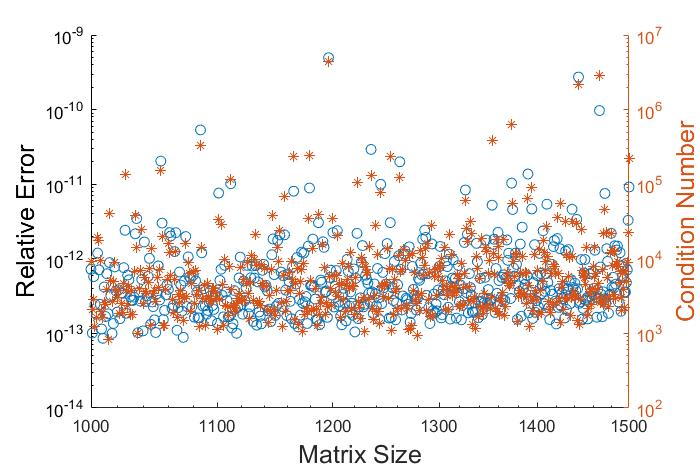
\includegraphics[width=0.48\linewidth]{code/prob2a.jpg}}   
   {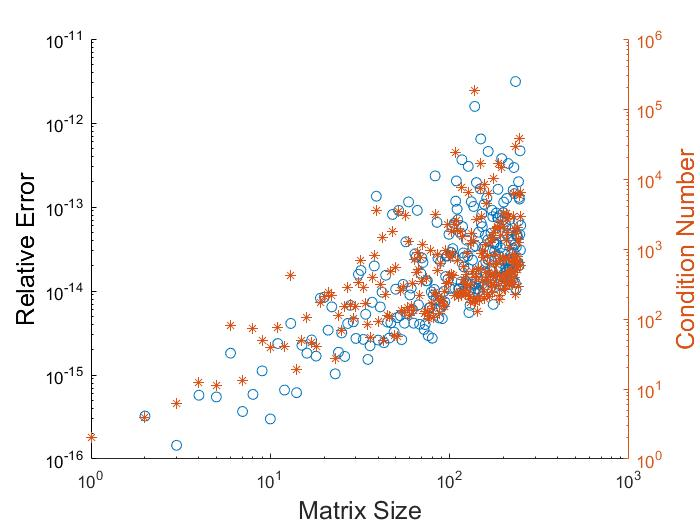
\includegraphics[width=0.48\linewidth]{code/prob2b.jpg}}
  \caption{Scatter plots for the relative error and conditions on log-log scale for different random matrices of different sizes.}
   \label{fig:sac}
\end{figure} 